\chapter{Metodologia badań} \label{chap.technology-stack}
\section{Opis metodologii badań}
Metodologia badań składa się z następujących elementów:
\begin{itemize}
	\item pobranie danych strumieniowych z serwisu Twitter,
	\item zapis danych w systemie HDFS,
	\item połączenie zapisanych wcześniej danych w jedno źródło danych masowych o wielkości 4GB,
	\item wykonanie jednej z operacji: \textit{WordCount, Filter, Reject} (\ref{e2e_operations}) na platformie Apache Hadoop oraz Apache Spark,
	\item pomiar wyników wydajności dla każdej operacji w odizolowanym, jednorodnym środowisku (szczegółowy opis jednostek pomiarów znajduje się w sekcji \ref{items:time-descriptions}),
	\item interpretacji rezultatów.
\end{itemize}
Dzięki takiej strategii postępowania można było dokonać skutecznego porównania ze względu na wydajność i stwierdzić, która platforma jest szybsza w przypadku zdefiniowanej specyfikacji sprzętowej oraz identycznego źródła danych. Kolejnym czynnikiem uwzględnionym podczas badań był sam kod źródłowy, który może stanowić o decyzji, które narzędzie wybrać. W szczególności rozważana została empiryczna złożoność kodu źródłowego, zarobki inżynierów ze względu na znajomość języka programowania oraz platform do przetwarzania danych masowych, środowisko rozwijania oprogramowania - duże projekty korporacyjne kontra małe aplikacje tworzone na zamówienie bez zapewnienia długofalowego wsparcia. Szczegóły badań drugiego czynniku są przedstawione w sekcji \ref{development_human_resources}.  
\section{Środowisko badań}
Do wykonania badań powstała aplikacja internetowa, która udostępnia końcowemu użytkownikowi protokół HTTP. Dzięki temu użytkownik może wykonywać operacje wykorzystujące paradygmat map-reduce bez znajomości platform udostępniających przetwarzanie danych masowych jak również serwisów internetowych. Aplikacja nosi nazwę \textit{big-data-runner}. Aplikacja może być udostępniona na zdalnym serwerze jak również może być uruchomiona lokalnie. Aby uruchomić aplikację jedyne co użytkownik musi posiadać to:
\begin{itemize}
	\item{wirtualna Maszyna Java w wersji 8\footnote{JVM \url{https://www.java.com/pl/download/}}},
	\item{Scala Build Tool \footnote{SBT \url{http://www.scala-sbt.org/}}}.
\end{itemize}
JVM jest odpowiedzialna za środowisko uruchomieniowe aplikacji internetowej. SBT to narzędzie, które umożliwia kompilację całej aplikacji wraz z bibliotekami zewnętrznymi (jeżeli biblioteki nie znajdują się w katalogu lokalnym zostaną pobrane ze zdalnego repozytorium) oraz jej uruchomienie w serwerze aplikacji internetowych \textit{Netty}\footnote{\url{https://netty.io/}}. Z ramę projektową odpowiedzialny jest Play Framework, który umożliwia łatwą i szybką implementację protokołu HTTP dla końcowego użytkownika.
\newpage
Zastosowane języki programowania to:
\begin{itemize}
	\item {Java},
	\item {Scala}.
\end{itemize}

Większość kodu aplikacji jest napisana w języku Scala - kontrolery, konfiguracja SBT, dostępy do serwisów zewnętrznych oraz wywoływanie interfejsu programistycznego Spark. Java została wykorzystana podczas obsługi API\footnote{Application Programmer Interface} platformy Hadoop tworząc w ten sposób własne API, które mogło być wykorzystane w kontrolerach napisanych w języku Scala.

\section{Architektura aplikacji}
Architektura aplikacji big-data-runner jest przedstawiona na rysunku \ref{fig:@=big-data-runner_arch}. 
\begin{figure}[!htb]
	\centering
	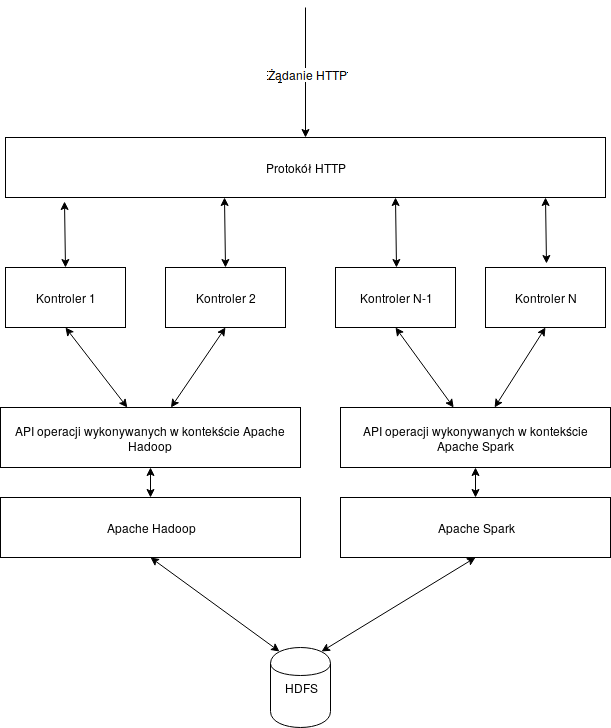
\includegraphics[scale=0.4]{big-data-runner-architecture.png}
	\caption{Architektura big-data-runner [źródło: Opracowanie własne].}
	\label{fig:@=big-data-runner_arch}
\end{figure}
\newline Podczas użytkowania użytkownik wysyła żądanie HTTP do aplikacji. Cały mechanizm obsługi żądania oraz odpowiedzi jest zaimplementowany w ramie projektowej Play! Za żądania odpowiedzialne są kontrolery, które wykonują logikę biznesową aplikacji. W zależności od adresu żądania wywołanego przez użytkownika uruchamiany jest odpowiedni kontroler, który wywołuje daną operację na platformie obliczeniowej. W zależności od tego, czy operacje są wywoływane w kontekście platformy Hadoop czy Spark, używane są odpowiednio języki programowania: Java, Scala. Z racji iż aplikacja integruje dwie platformy obok siebie możemy uznać, że kontrolery są częścią aplikacji, które wysyłają \textit{driver program}\footnote{Program sterujący - \url{http://spark.apache.org/docs/latest/cluster-overview.html}} do platformy Hadoop lub Spark. W dokumentacji Apache Hadoop możemy spotkać się z określeniem \textit{Job Configuration}\footnote{Konfiguracja pracy - \url{https://hadoop.apache.org/docs/r2.7.3/api/org/apache/hadoop/mapreduce/Job.html}}. Po wysłaniu odpowiednich instrukcji następuje wykonywanie obliczeń przez daną platformę. Same platformy są dołączone do aplikacji jako biblioteki zewnętrzne. Są integrowane przez narzędzie budujące aplikację SBT. Jednym elementem systemu przetwarzania danych masowych, który nie jest zintegrowany z aplikacją jest HDFS - warstwa odpowiedzialna za przechowywanie danych. HDFS może być umiejscowiony na zdalnym serwerze bądź obok samej aplikacji. Może być pobrany pod adresem: \url{http://hadoop.apache.org/releases.html}. W przeprowadzonych badaniach została użyta wersja 2.8.0. Adres HDFS jest zdefiniowany we właściwościach aplikacji, które znajdują się w pliku \path{<application-root>/conf/application.conf}. Dzięki temu w łatwy sposób administrator aplikacji może zmieniać adres źródła danych.
\section{Interfejs końcowy użytkownika}\label{sec:user_interfaces}
Żądania HTTP obsługują trzy rodzaje operacji, które można wykonać na platformach równoległych:
\begin{itemize}\label{e2e_operations}
	\item {zliczanie ilości wystąpień poszczególnych fraz tekstowych (oddzielonych spacją) znalezionych w źródle danych oraz zapisu wyniku do pliku}\footnote{\textit{Word Count}},
	\item {zliczanie ilości linii zawierających frazę tekstową zdefiniowaną przez użytkownika}\footnote{\textit{Filter}},
	\item {odrzucenie linii zawierających frazę tekstową zdefiniowaną przez użytkownika oraz zapisanie wyniku do pliku}\footnote{\textit{Reject}}.
\end{itemize}
Użytkownik może wybrać następujące punkty obsługi żądania:
\begin{enumerate}
	\item{\url{<hostname>/api/spark/wordcount}}
	\item{\url{<hostname>/api/spark/wordOccurrence/<string> }}
	\item{\url{<hostname>/api/spark/wordReject/<string> }}
	\item{\url{<hostname>/api/hadoop/wordcount}}
	\item{\url{<hostname>/api/hadoop/wordOccurrence/<string>}}
	\item{\url{<hostname>/api/hadoop/wordReject/<string> }}
\end{enumerate}
Punkty od 1 do 3 obsługują platformę Spark. Punkt 1 jest odpowiedzialny za zliczanie wystąpień poszczególnych fraz, punkt 2 za zliczanie wystąpień danej frazy w linii. Punkt 3 odrzuca te linie, które zawierały frazę zdefiniowaną przez użytkownika. Odpowiednio punkty 4, 5, 6 są odpowiedzialne za te same operacje z tą różnicą, że są uruchamiane na platformie Hadoop.  

\section{Dostęp do serwisów zewnętrznych}\label{sec:twitter-api}
Aplikacja posiada również dostęp do jednego serwisu zewnętrznego jakim jest \textit{Twitter Developer API}\footnote{\url{https://dev.twitter.com/}}. Funkcjonalność ta została zaimplementowana, gdyż Twitter jest doskonałym źródłem danych masowych. Na podstawie danych zebranych poprzez Twitter Developer API zostały wykonane badania dotyczące szybkości obu platform. Sam proces zbierania danych jest zaimplementowany poprzez wykorzystanie \textit{Spark Streaming}\footnote{\url{http://spark.apache.org/streaming/}}. Dzięki temu użytkownik jest w stanie zbierać dane "na żywo". Oznacza to, że otwierany jest potok z danymi, które są zapisywane cyklicznie do HDFS. Cykl zapisu to okres czasu co jaki ma wystąpić zapis. W przypadku aplikacji big-data-runner jest to \textbf{360 sekund}. Dzięki takiemu podejściu możliwe jest zbieranie wielkich ilości danych bez ryzyka, iż niestabilne połączenie internetowe uszkodzi dane, bądź całkowicie uniemożliwi zapis. Aby móc skorzystać z Twitter Developer API wymagane są odpowiednie uprawnienia. Uprawnienia są przyznawane dla pary: użytkownik - aplikacja. Dane uprawnień znajdują się w pliku \path{<application-root>/conf/twitter.conf}. Konfiguracja uprawnień jest zapewniona przez bibliotekę \textit{Twitter4J}.\footnote{\url{http://twitter4j.org}}
\newline Dane mogą być zbierane poprzez dwa punkty obsługi żądania aplikacji:
\begin{enumerate}
	\item{\url{<hostname>/api/spark/live/list/start}}
	\item{\url{<hostname>/api/spark/live/list/stop}}
\end{enumerate}
Punkt nr 1 odpowiada za wystartowanie strumieniowania danych do HDFS skonfigurowanego z aplikacją. Punkt nr 2 kończy operację strumieniowania. Zakończenie strumieniowania nie jest natychmiastowe, aplikacja czeka aż cykl zapisu zostanie ukończony. Zasada działania jest taka sama jak w przypadku punktów obsługi wymienionych w sekcji \ref{sec:user_interfaces} z jednym wyjątkiem - przed zatwierdzeniem operacji na platformie Spark, wykonywana jest konfiguracja dostępu do Twitter Developer API. Następnie rozpoczyna się strumieniowanie danych.

\section{Źródła danych}
Podczas badań zostały przeprowadzone testy wydajności dla trzech operacji, które są reprezentowane przez końcowy interfejs użytkownika. Dokładny opis dostępu do danych jak i ich struktury znajduje się w sekcji \ref{sec:twitter-api} oraz \ref{sec:tweet-structure}. Szczegółowa definicja operacji znajduję się w sekcji \ref{sec:user_interfaces}. 
Na potrzeby badań operacje nazwijmy następująco:
\begin{itemize}
	\item {Word Count}
	\item {Filter}
	\item {Reject}
\end{itemize}
Testy wydajności zostały wykonane na danych zebranych poprzez Twitter Developer API opisanym w sekcji \ref{sec:twitter-api}. Z racji iż strumieniowanie dla platformy Spark zapisuje dane cyklicznie, powstał katalog w systemie HDFS zawierający paczki danych zapisanych co 360 sekund. Na potrzeby badań wszystkie dane pobrane ze zdalnego API zostały połączone w jeden plik o wielkości \textbf{4GB}, który posłużył za źródło danych podczas wykonywania testów wydajności. Twitter Developer API nie jest standardowym webowym interfejsem typu REST\footnote{Representational state transfer}. Nie występuje tutaj standardowy scenariusz zapytanie do serwera, odpowiedź serwera. W przypadku danych strumieniowych, klient wysyła zapytanie do aplikacji, aplikacja wysyła zapytanie do serwerów Twitter i czeka na odpowiedź serwera asynchronicznie. Klient wysyłając jedynie żądanie nie blokuje samego interfejsu aplikacji. W związku z tym może występować złudzenie iż klient nie posiada kontroli nad samym pobieraniem danych, gdyż raz wysłane żądanie nie może zostać przerwane. Aplikacja sama zarządza procesem pobierania/strumieniowania danych. Architektura o podobnej strategii jest proponowana również przez twórców samego Twitter Developer API i jest zaprezentowana na pod adresem: \url{https://dev.twitter.com/streaming/overview}.
\begin{figure}
	\centering
	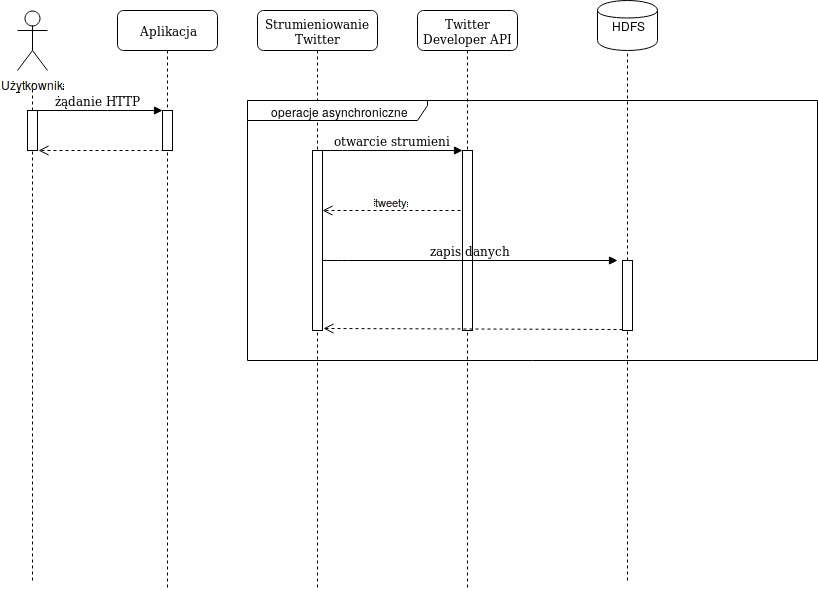
\includegraphics[scale=0.5]{twitter-api-connection.png}
	\caption{Architektura procesu pobierania danych z Twitter Developer API [źródło: Opracowanie własne].}
	\label{fig:@=twitter-api-connection}
\end{figure}
Proces strumieniowania danych z Twitter Developer API został przedstawiony na rysunku \ref{fig:@=twitter-api-connection}.
\section{Struktura źródeł danych}\label{sec:tweet-structure}
Dane pobrane z Twitter Developer API są zapisywane w systemie plików HDFS, do którego dostęp jest skonfigurowany wewnątrz głównej aplikacji. Adres dostępu do systemu HDFS może być modyfikowany przez administratora aplikacji i znajduje się w pliku \url{<application-root>./conf/application.conf}. Dane są przyjmowane jako \textit{DStream}\footnote{Discretized Stream}, który jest główną warstwą abstrakcji dla strumieniowania danych. Wewnętrznie jest to ciąg stale napływających danych w formule RDD, szczegóły na temat RDD można znaleźć w sekcji \ref{rdd-section}. Następnie na napływających danych jest wywołana funkcja \textit{map}, która zapisuje równolegle rozproszony zbiór danych w systemie HDFS. Zapisanie jest dokonane w formacie JSON\footnote{JavaScript Object Notation}. JSON został wybrany ze względu na prostą strukturę i przystępną dla ludzkiego oka prezentację. Otwarcie strumieniowania jest przestawione w listingu \ref{lst:twitter-streaming-scala}  
\begin{lstlisting}[language=scala, caption={Otwarcie strumieniowania Twitter Developer API oraz zapis do HDFS},captionpos=b, label={lst:twitter-streaming-scala}]
val twitterInstance = new Twitter4JConfiguration(config).getTwitter4JAccess()
val tweetStream = TwitterUtils.createStream(SparkStreaming.streamingContext, Option(twitterInstance.getAuthorization)).map(new Gson().toJson(_))
tweetStream.foreachRDD((rdd, time) => {
val outputRDD = rdd.repartition(4)
outputRDD.saveAsTextFile(config.getString("hadoop-tweets-url").get + "tweet_" + time.milliseconds.toString)
})
SparkStreaming.streamingContext.start()
\end{lstlisting}
W linii nr 1 następuje konfiguracja dostępu do Twitter Developer API przy użyciu biblioteki Twitter4J\footnote{\url{http://twitter4j.org}}. Linia nr 2 to deklaracja strumienia, ustawienia autoryzacji dla Twitter Developer API oraz konfiguracja formatu zapisu danych. Linie nr 3,4,5 to konfiguracja samego zapisu w systemie HDFS, ustalana jest ilość partycji, na których ma zostać zapisane RDD oraz jak ma nazywać się wynikowy plik w HDFS. Linia nr 8 rozpoczyna faktyczne strumieniowanie danych oraz ich zapis.
\newline Struktura danych zwracana z Twitter Developer API w formacie JSON zawiera bardzo dużo informacji. Jedne z najbardziej kluczowych są przedstawione w liście \ref{items:tweet-fields}
\begin{itemize}\label{items:tweet-fields}
	\item data utworzenia\footnote{createdAt},
	\item udostępnienia tweet'a \footnote{retweetedStatus},
	\item zawartość tweet'a\footnote{text},
	\item autor\footnote{user},
	\item flaga prawda/fałsz dotycząca treści wrażliwych\footnote{isPossiblySensitive}.
\end{itemize}
Dokładna struktura danych jest przedstawiona w listingu: \ref{lst:tweet-json}
\lstinputlisting[language=json,firstnumber=1, label={lst:tweet-json}, captionpos=b, caption={Przykładowa struktura danych pobrana z Twitter Developer API, użyta podczas badań.}]{tweet.json}  
\section{Specyfikacja sprzętowa i konfiguracja platform}
Badania zostały przeprowadzone na maszynie o specyfikacji:
\begin{itemize}
	\item Procesor: Intel Core i7-4702MQ (2.2GHz Quad-core + HT) 
	\item Pamięć RAM: 16GB
	\item Pamięć masowa: 1 TB 5400rpm\footnote{Revolutions per minute - obroty na minutę} SATA
	\item Karta graficzna: NVIDIA GeForce GT 750M (2G)  
\end{itemize}
Podczas badań specyfikacja karty graficznej nie ma wpływu na wyniki, gdyż dla badanych operacji wykorzystywane są trzy jednostki obliczeniowe: procesor, pamięć RAM, dysk twardy.
\newline Pomiary wydajności zostały dokonane przy pomocy programu \textbf{cURL}.\footnote{\url{https://curl.haxx.se/}} Testy obejmują siedem następujących czynników:
\begin{itemize}\label{items:time-descriptions}
	\item{Czas rozwiązywania adresu\footnote{time\_namelookup}}
	\item{Czas połączenia TCP\footnote{time\_connect}}
	\item{Czas wymiany informacji między połączeniami (handshake)\footnote{time\_appconnect}} 
	\item{Czas całkowity przed wymianą informacji\footnote{time\_pretransfer}}
	\item{Czas przekierowań\footnote{time\_redirect}}
	\item{Czas przed którym pierwszy bajt danych miał zostać wysłany\footnote{time\_starttransfer}}
	\item{Czas całkowity\footnote{time\_total}}
\end{itemize}
Obydwie platformy pozwalają na szczegółową konfigurację instalacji. Z racji, iż testy były wykonywane na jednej i tej samej maszynie należało ustawić sztuczny(wirtualny) klaster. Oznacza to, że na maszynie było imitowane rozproszone środowisko obliczeniowe. Dla Apache Spark tryb lokalny został ustawiony na maksymalną możliwą liczbę dostępnych wątków wirtualnej maszyny Java - oznacza to, że liczba zwróconych dostępnych wątków przez metodę przedstawioną na listingu \ref{lst:jvm-threads-access} definiuje ile operacji Apache Spark może wykonywać w tej samej jednostce czasu. Konfiguracja jest widoczna na listingu \ref{lst:spark-cluster-config}. Konfiguracja pozwala na tworzenie kontekstu dla zapytań o dane statyczne (na przykład baza danych), jak również o charakterze dynamicznym (strumieniowanie). Jak widać na listingu \ref{lst:spark-cluster-config} w linii 4 ustawiany jest również cykl zapisu danych dynamicznych (zapis co 360 sekund).
\begin{lstlisting}[language=scala, caption={Metoda zwracająca liczbę dostępnych wątków wirtualnej maszyny Java},captionpos=b, label={lst:jvm-threads-access}]
Runtime.getRuntime.availableProcessors() 
\end{lstlisting}
\begin{lstlisting}[language=scala, caption={Konfigracja klastra dla Apache Spark},captionpos=b, label={lst:spark-cluster-config}]
object SparkStreaming {
val conf = new SparkConf().setMaster("local[*]").setAppName("big-data-runner-spark-driver-application")
val sparkContext = new SparkContext(conf)
val streamingContext = new StreamingContext(sparkContext, Seconds(360))
}
\end{lstlisting} 
Apache Hadoop może być uruchamiany w trzech trybach: pojedynczy proces JVM (\textit{Standalone Operation)}, pseudo rozproszony \textit{Pseudo-Distributed Operation}, w pełni rozproszony \textit{Fully-Distributed Operation}. Aby konfiguracja była jak najbardziej podobna do konfiguracji Spark, Hadoop został uruchomiony w trybie pseudo rozproszonym. W takim przypadku Apache Hadoop nie jest konfigurowany przez kod źródłowy, lecz przez pliki konfiguracyjne XML. Konfiguracja Apache Hadoop jest przedstawiona na listingach \ref{lst:core-site} i \ref{lst:hdfs-site}.
\begin{lstlisting}[language=XML, label={lst:hdfs-site},captionpos=b, caption={Konfigracja Apache Hadoop dla trybu pseudo rozproszonego. Plik hdfs-site.xml}]
<configuration>
<property>
<name>dfs.replication</name>
<value>4</value>
</property>
</configuration>
\end{lstlisting}
\begin{lstlisting}[language=XML, label={lst:core-site}, captionpos=b, caption={Konfigracja Apache Hadoop dla trybu pseudo rozproszonego. Plik core-site.xml}, float]
<configuration>
<property>
<name>fs.defaultFS</name>
<value>hdfs://127.0.0.1:8080</value>
</property>
<property>
<name>hadoop.tmp.dir</name>
<value>/home/szymonidas/tweets-hdfs/</value>
</property>
</configuration>
\end{lstlisting}
Poza adresem Apache Hadoop, został zdefiniowany katalog na dysku twardym, gdzie HDFS będzie przechowywał swoje dane. Hadoop podobnie jak Spark został ustawiony na partycjonowanie danych w czterech częściach.
